% Created by tikzDevice version 0.11 on 2018-07-18 22:48:11
% !TEX encoding = UTF-8 Unicode
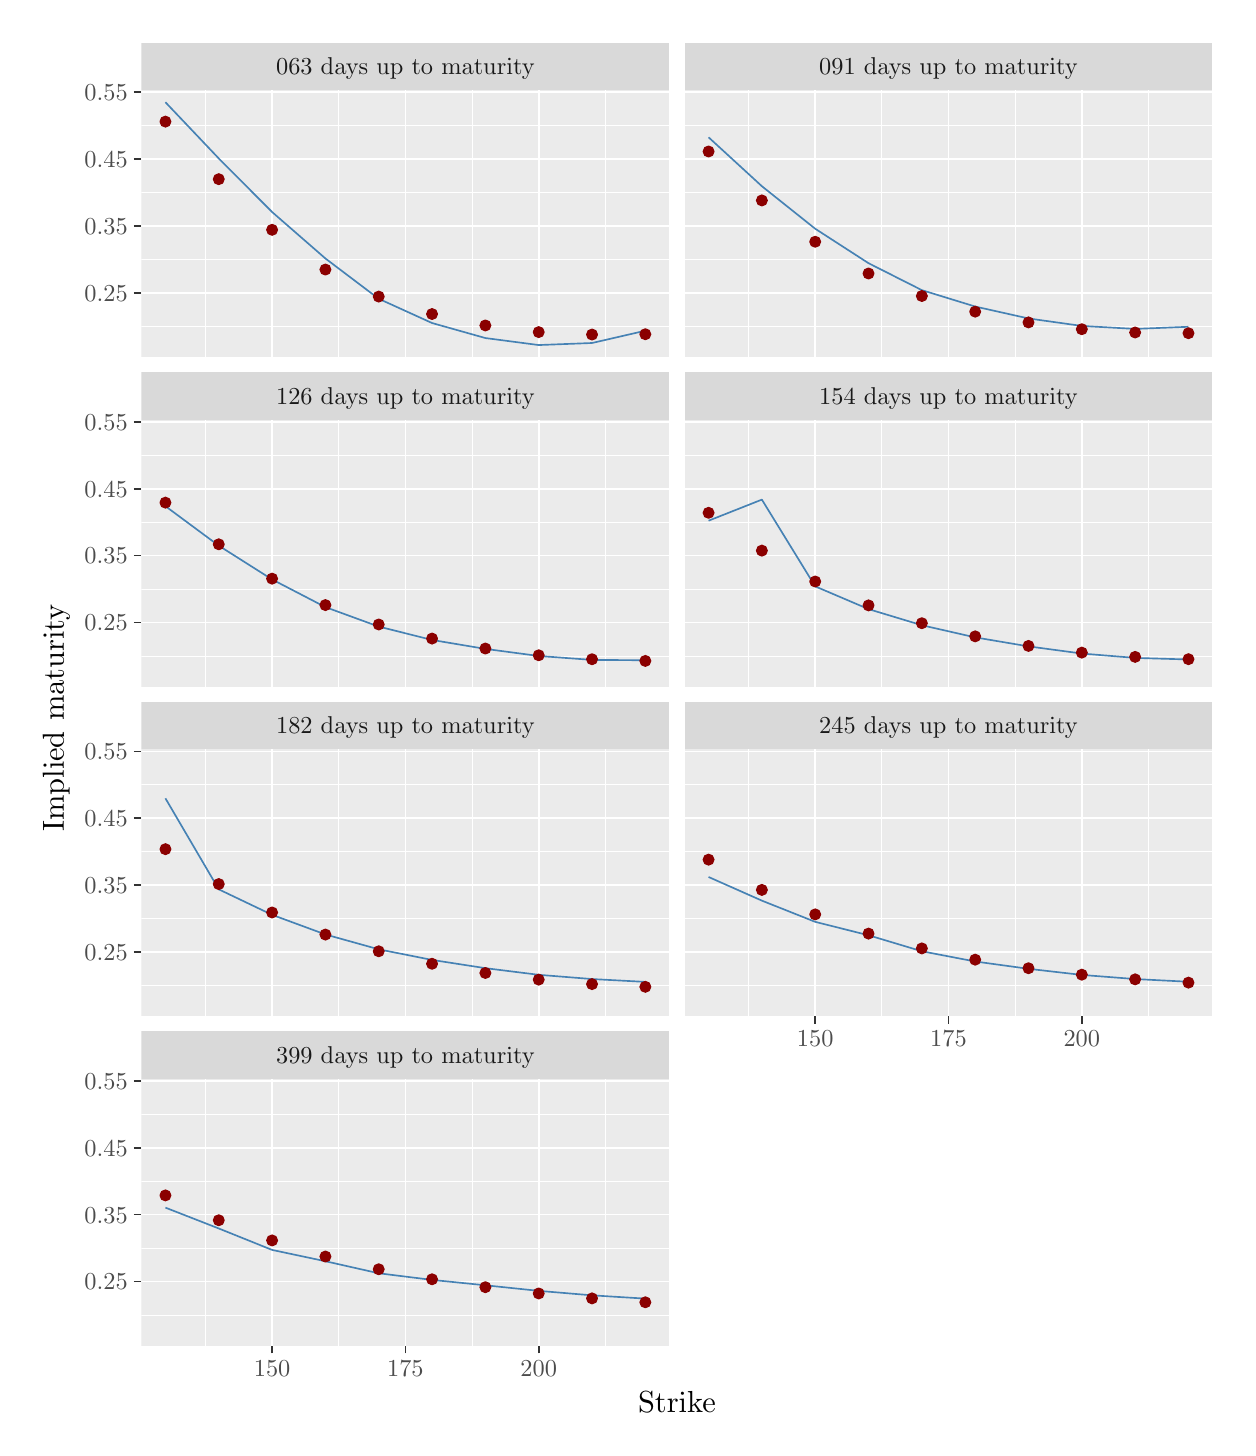
\begin{tikzpicture}[x=1pt,y=1pt]
\definecolor{fillColor}{RGB}{255,255,255}
\path[use as bounding box,fill=fillColor,fill opacity=0.00] (0,0) rectangle (433.62,505.89);
\begin{scope}
\path[clip] (  0.00,  0.00) rectangle (433.62,505.89);
\definecolor{drawColor}{RGB}{255,255,255}
\definecolor{fillColor}{RGB}{255,255,255}

\path[draw=drawColor,line width= 0.6pt,line join=round,line cap=round,fill=fillColor] (  0.00,  0.00) rectangle (433.62,505.89);
\end{scope}
\begin{scope}
\path[clip] ( 41.11,386.81) rectangle (231.87,483.33);
\definecolor{fillColor}{gray}{0.92}

\path[fill=fillColor] ( 41.11,386.81) rectangle (231.87,483.33);
\definecolor{drawColor}{RGB}{255,255,255}

\path[draw=drawColor,line width= 0.3pt,line join=round] ( 41.11,397.93) --
	(231.87,397.93);

\path[draw=drawColor,line width= 0.3pt,line join=round] ( 41.11,422.11) --
	(231.87,422.11);

\path[draw=drawColor,line width= 0.3pt,line join=round] ( 41.11,446.28) --
	(231.87,446.28);

\path[draw=drawColor,line width= 0.3pt,line join=round] ( 41.11,470.45) --
	(231.87,470.45);

\path[draw=drawColor,line width= 0.3pt,line join=round] ( 64.23,386.81) --
	( 64.23,483.33);

\path[draw=drawColor,line width= 0.3pt,line join=round] (112.40,386.81) --
	(112.40,483.33);

\path[draw=drawColor,line width= 0.3pt,line join=round] (160.57,386.81) --
	(160.57,483.33);

\path[draw=drawColor,line width= 0.3pt,line join=round] (208.74,386.81) --
	(208.74,483.33);

\path[draw=drawColor,line width= 0.6pt,line join=round] ( 41.11,410.02) --
	(231.87,410.02);

\path[draw=drawColor,line width= 0.6pt,line join=round] ( 41.11,434.19) --
	(231.87,434.19);

\path[draw=drawColor,line width= 0.6pt,line join=round] ( 41.11,458.37) --
	(231.87,458.37);

\path[draw=drawColor,line width= 0.6pt,line join=round] ( 41.11,482.54) --
	(231.87,482.54);

\path[draw=drawColor,line width= 0.6pt,line join=round] ( 88.32,386.81) --
	( 88.32,483.33);

\path[draw=drawColor,line width= 0.6pt,line join=round] (136.49,386.81) --
	(136.49,483.33);

\path[draw=drawColor,line width= 0.6pt,line join=round] (184.66,386.81) --
	(184.66,483.33);
\definecolor{drawColor}{RGB}{70,130,180}

\path[draw=drawColor,line width= 0.6pt,line join=round] ( 49.78,478.94) --
	( 69.05,458.63) --
	( 88.32,439.27) --
	(107.59,422.48) --
	(126.85,407.92) --
	(146.12,399.16) --
	(165.39,393.73) --
	(184.66,391.20) --
	(203.93,391.94) --
	(223.19,396.38);
\definecolor{drawColor}{RGB}{139,0,0}
\definecolor{fillColor}{RGB}{139,0,0}

\path[draw=drawColor,line width= 0.4pt,line join=round,line cap=round,fill=fillColor] ( 49.78,471.94) circle (  1.96);

\path[draw=drawColor,line width= 0.4pt,line join=round,line cap=round,fill=fillColor] ( 69.05,451.14) circle (  1.96);

\path[draw=drawColor,line width= 0.4pt,line join=round,line cap=round,fill=fillColor] ( 88.32,432.84) circle (  1.96);

\path[draw=drawColor,line width= 0.4pt,line join=round,line cap=round,fill=fillColor] (107.59,418.48) circle (  1.96);

\path[draw=drawColor,line width= 0.4pt,line join=round,line cap=round,fill=fillColor] (126.85,408.72) circle (  1.96);

\path[draw=drawColor,line width= 0.4pt,line join=round,line cap=round,fill=fillColor] (146.12,402.41) circle (  1.96);

\path[draw=drawColor,line width= 0.4pt,line join=round,line cap=round,fill=fillColor] (165.39,398.28) circle (  1.96);

\path[draw=drawColor,line width= 0.4pt,line join=round,line cap=round,fill=fillColor] (184.66,395.88) circle (  1.96);

\path[draw=drawColor,line width= 0.4pt,line join=round,line cap=round,fill=fillColor] (203.93,394.99) circle (  1.96);

\path[draw=drawColor,line width= 0.4pt,line join=round,line cap=round,fill=fillColor] (223.19,395.11) circle (  1.96);
\end{scope}
\begin{scope}
\path[clip] ( 41.11,267.74) rectangle (231.87,364.25);
\definecolor{fillColor}{gray}{0.92}

\path[fill=fillColor] ( 41.11,267.74) rectangle (231.87,364.25);
\definecolor{drawColor}{RGB}{255,255,255}

\path[draw=drawColor,line width= 0.3pt,line join=round] ( 41.11,278.86) --
	(231.87,278.86);

\path[draw=drawColor,line width= 0.3pt,line join=round] ( 41.11,303.03) --
	(231.87,303.03);

\path[draw=drawColor,line width= 0.3pt,line join=round] ( 41.11,327.20) --
	(231.87,327.20);

\path[draw=drawColor,line width= 0.3pt,line join=round] ( 41.11,351.38) --
	(231.87,351.38);

\path[draw=drawColor,line width= 0.3pt,line join=round] ( 64.23,267.74) --
	( 64.23,364.25);

\path[draw=drawColor,line width= 0.3pt,line join=round] (112.40,267.74) --
	(112.40,364.25);

\path[draw=drawColor,line width= 0.3pt,line join=round] (160.57,267.74) --
	(160.57,364.25);

\path[draw=drawColor,line width= 0.3pt,line join=round] (208.74,267.74) --
	(208.74,364.25);

\path[draw=drawColor,line width= 0.6pt,line join=round] ( 41.11,290.95) --
	(231.87,290.95);

\path[draw=drawColor,line width= 0.6pt,line join=round] ( 41.11,315.12) --
	(231.87,315.12);

\path[draw=drawColor,line width= 0.6pt,line join=round] ( 41.11,339.29) --
	(231.87,339.29);

\path[draw=drawColor,line width= 0.6pt,line join=round] ( 41.11,363.46) --
	(231.87,363.46);

\path[draw=drawColor,line width= 0.6pt,line join=round] ( 88.32,267.74) --
	( 88.32,364.25);

\path[draw=drawColor,line width= 0.6pt,line join=round] (136.49,267.74) --
	(136.49,364.25);

\path[draw=drawColor,line width= 0.6pt,line join=round] (184.66,267.74) --
	(184.66,364.25);
\definecolor{drawColor}{RGB}{70,130,180}

\path[draw=drawColor,line width= 0.6pt,line join=round] ( 49.78,332.98) --
	( 69.05,318.71) --
	( 88.32,306.50) --
	(107.59,296.51) --
	(126.85,289.47) --
	(146.12,284.64) --
	(165.39,281.41) --
	(184.66,278.85) --
	(203.93,277.43) --
	(223.19,277.30);
\definecolor{drawColor}{RGB}{139,0,0}
\definecolor{fillColor}{RGB}{139,0,0}

\path[draw=drawColor,line width= 0.4pt,line join=round,line cap=round,fill=fillColor] ( 49.78,334.26) circle (  1.96);

\path[draw=drawColor,line width= 0.4pt,line join=round,line cap=round,fill=fillColor] ( 69.05,319.20) circle (  1.96);

\path[draw=drawColor,line width= 0.4pt,line join=round,line cap=round,fill=fillColor] ( 88.32,306.79) circle (  1.96);

\path[draw=drawColor,line width= 0.4pt,line join=round,line cap=round,fill=fillColor] (107.59,297.24) circle (  1.96);

\path[draw=drawColor,line width= 0.4pt,line join=round,line cap=round,fill=fillColor] (126.85,290.23) circle (  1.96);

\path[draw=drawColor,line width= 0.4pt,line join=round,line cap=round,fill=fillColor] (146.12,285.14) circle (  1.96);

\path[draw=drawColor,line width= 0.4pt,line join=round,line cap=round,fill=fillColor] (165.39,281.54) circle (  1.96);

\path[draw=drawColor,line width= 0.4pt,line join=round,line cap=round,fill=fillColor] (184.66,279.10) circle (  1.96);

\path[draw=drawColor,line width= 0.4pt,line join=round,line cap=round,fill=fillColor] (203.93,277.67) circle (  1.96);

\path[draw=drawColor,line width= 0.4pt,line join=round,line cap=round,fill=fillColor] (223.19,277.06) circle (  1.96);
\end{scope}
\begin{scope}
\path[clip] ( 41.11,148.66) rectangle (231.87,245.18);
\definecolor{fillColor}{gray}{0.92}

\path[fill=fillColor] ( 41.11,148.66) rectangle (231.87,245.18);
\definecolor{drawColor}{RGB}{255,255,255}

\path[draw=drawColor,line width= 0.3pt,line join=round] ( 41.11,159.78) --
	(231.87,159.78);

\path[draw=drawColor,line width= 0.3pt,line join=round] ( 41.11,183.96) --
	(231.87,183.96);

\path[draw=drawColor,line width= 0.3pt,line join=round] ( 41.11,208.13) --
	(231.87,208.13);

\path[draw=drawColor,line width= 0.3pt,line join=round] ( 41.11,232.30) --
	(231.87,232.30);

\path[draw=drawColor,line width= 0.3pt,line join=round] ( 64.23,148.66) --
	( 64.23,245.18);

\path[draw=drawColor,line width= 0.3pt,line join=round] (112.40,148.66) --
	(112.40,245.18);

\path[draw=drawColor,line width= 0.3pt,line join=round] (160.57,148.66) --
	(160.57,245.18);

\path[draw=drawColor,line width= 0.3pt,line join=round] (208.74,148.66) --
	(208.74,245.18);

\path[draw=drawColor,line width= 0.6pt,line join=round] ( 41.11,171.87) --
	(231.87,171.87);

\path[draw=drawColor,line width= 0.6pt,line join=round] ( 41.11,196.04) --
	(231.87,196.04);

\path[draw=drawColor,line width= 0.6pt,line join=round] ( 41.11,220.21) --
	(231.87,220.21);

\path[draw=drawColor,line width= 0.6pt,line join=round] ( 41.11,244.39) --
	(231.87,244.39);

\path[draw=drawColor,line width= 0.6pt,line join=round] ( 88.32,148.66) --
	( 88.32,245.18);

\path[draw=drawColor,line width= 0.6pt,line join=round] (136.49,148.66) --
	(136.49,245.18);

\path[draw=drawColor,line width= 0.6pt,line join=round] (184.66,148.66) --
	(184.66,245.18);
\definecolor{drawColor}{RGB}{70,130,180}

\path[draw=drawColor,line width= 0.6pt,line join=round] ( 49.78,227.41) --
	( 69.05,194.52) --
	( 88.32,185.32) --
	(107.59,178.22) --
	(126.85,172.85) --
	(146.12,169.02) --
	(165.39,166.04) --
	(184.66,163.64) --
	(203.93,162.11) --
	(223.19,161.08);
\definecolor{drawColor}{RGB}{139,0,0}
\definecolor{fillColor}{RGB}{139,0,0}

\path[draw=drawColor,line width= 0.4pt,line join=round,line cap=round,fill=fillColor] ( 49.78,209.04) circle (  1.96);

\path[draw=drawColor,line width= 0.4pt,line join=round,line cap=round,fill=fillColor] ( 69.05,196.43) circle (  1.96);

\path[draw=drawColor,line width= 0.4pt,line join=round,line cap=round,fill=fillColor] ( 88.32,186.16) circle (  1.96);

\path[draw=drawColor,line width= 0.4pt,line join=round,line cap=round,fill=fillColor] (107.59,178.18) circle (  1.96);

\path[draw=drawColor,line width= 0.4pt,line join=round,line cap=round,fill=fillColor] (126.85,172.14) circle (  1.96);

\path[draw=drawColor,line width= 0.4pt,line join=round,line cap=round,fill=fillColor] (146.12,167.63) circle (  1.96);

\path[draw=drawColor,line width= 0.4pt,line join=round,line cap=round,fill=fillColor] (165.39,164.30) circle (  1.96);

\path[draw=drawColor,line width= 0.4pt,line join=round,line cap=round,fill=fillColor] (184.66,161.90) circle (  1.96);

\path[draw=drawColor,line width= 0.4pt,line join=round,line cap=round,fill=fillColor] (203.93,160.28) circle (  1.96);

\path[draw=drawColor,line width= 0.4pt,line join=round,line cap=round,fill=fillColor] (223.19,159.30) circle (  1.96);
\end{scope}
\begin{scope}
\path[clip] ( 41.11, 29.59) rectangle (231.87,126.10);
\definecolor{fillColor}{gray}{0.92}

\path[fill=fillColor] ( 41.11, 29.59) rectangle (231.87,126.10);
\definecolor{drawColor}{RGB}{255,255,255}

\path[draw=drawColor,line width= 0.3pt,line join=round] ( 41.11, 40.71) --
	(231.87, 40.71);

\path[draw=drawColor,line width= 0.3pt,line join=round] ( 41.11, 64.88) --
	(231.87, 64.88);

\path[draw=drawColor,line width= 0.3pt,line join=round] ( 41.11, 89.05) --
	(231.87, 89.05);

\path[draw=drawColor,line width= 0.3pt,line join=round] ( 41.11,113.22) --
	(231.87,113.22);

\path[draw=drawColor,line width= 0.3pt,line join=round] ( 64.23, 29.59) --
	( 64.23,126.10);

\path[draw=drawColor,line width= 0.3pt,line join=round] (112.40, 29.59) --
	(112.40,126.10);

\path[draw=drawColor,line width= 0.3pt,line join=round] (160.57, 29.59) --
	(160.57,126.10);

\path[draw=drawColor,line width= 0.3pt,line join=round] (208.74, 29.59) --
	(208.74,126.10);

\path[draw=drawColor,line width= 0.6pt,line join=round] ( 41.11, 52.79) --
	(231.87, 52.79);

\path[draw=drawColor,line width= 0.6pt,line join=round] ( 41.11, 76.97) --
	(231.87, 76.97);

\path[draw=drawColor,line width= 0.6pt,line join=round] ( 41.11,101.14) --
	(231.87,101.14);

\path[draw=drawColor,line width= 0.6pt,line join=round] ( 41.11,125.31) --
	(231.87,125.31);

\path[draw=drawColor,line width= 0.6pt,line join=round] ( 88.32, 29.59) --
	( 88.32,126.10);

\path[draw=drawColor,line width= 0.6pt,line join=round] (136.49, 29.59) --
	(136.49,126.10);

\path[draw=drawColor,line width= 0.6pt,line join=round] (184.66, 29.59) --
	(184.66,126.10);
\definecolor{drawColor}{RGB}{70,130,180}

\path[draw=drawColor,line width= 0.6pt,line join=round] ( 49.78, 79.51) --
	( 69.05, 71.98) --
	( 88.32, 64.23) --
	(107.59, 60.14) --
	(126.85, 55.79) --
	(146.12, 53.40) --
	(165.39, 51.45) --
	(184.66, 49.44) --
	(203.93, 47.82) --
	(223.19, 46.63);
\definecolor{drawColor}{RGB}{139,0,0}
\definecolor{fillColor}{RGB}{139,0,0}

\path[draw=drawColor,line width= 0.4pt,line join=round,line cap=round,fill=fillColor] ( 49.78, 83.93) circle (  1.96);

\path[draw=drawColor,line width= 0.4pt,line join=round,line cap=round,fill=fillColor] ( 69.05, 74.95) circle (  1.96);

\path[draw=drawColor,line width= 0.4pt,line join=round,line cap=round,fill=fillColor] ( 88.32, 67.66) circle (  1.96);

\path[draw=drawColor,line width= 0.4pt,line join=round,line cap=round,fill=fillColor] (107.59, 61.84) circle (  1.96);

\path[draw=drawColor,line width= 0.4pt,line join=round,line cap=round,fill=fillColor] (126.85, 57.24) circle (  1.96);

\path[draw=drawColor,line width= 0.4pt,line join=round,line cap=round,fill=fillColor] (146.12, 53.62) circle (  1.96);

\path[draw=drawColor,line width= 0.4pt,line join=round,line cap=round,fill=fillColor] (165.39, 50.76) circle (  1.96);

\path[draw=drawColor,line width= 0.4pt,line join=round,line cap=round,fill=fillColor] (184.66, 48.50) circle (  1.96);

\path[draw=drawColor,line width= 0.4pt,line join=round,line cap=round,fill=fillColor] (203.93, 46.72) circle (  1.96);

\path[draw=drawColor,line width= 0.4pt,line join=round,line cap=round,fill=fillColor] (223.19, 45.31) circle (  1.96);
\end{scope}
\begin{scope}
\path[clip] (237.37,386.81) rectangle (428.12,483.33);
\definecolor{fillColor}{gray}{0.92}

\path[fill=fillColor] (237.37,386.81) rectangle (428.12,483.33);
\definecolor{drawColor}{RGB}{255,255,255}

\path[draw=drawColor,line width= 0.3pt,line join=round] (237.37,397.93) --
	(428.12,397.93);

\path[draw=drawColor,line width= 0.3pt,line join=round] (237.37,422.11) --
	(428.12,422.11);

\path[draw=drawColor,line width= 0.3pt,line join=round] (237.37,446.28) --
	(428.12,446.28);

\path[draw=drawColor,line width= 0.3pt,line join=round] (237.37,470.45) --
	(428.12,470.45);

\path[draw=drawColor,line width= 0.3pt,line join=round] (260.49,386.81) --
	(260.49,483.33);

\path[draw=drawColor,line width= 0.3pt,line join=round] (308.66,386.81) --
	(308.66,483.33);

\path[draw=drawColor,line width= 0.3pt,line join=round] (356.83,386.81) --
	(356.83,483.33);

\path[draw=drawColor,line width= 0.3pt,line join=round] (405.00,386.81) --
	(405.00,483.33);

\path[draw=drawColor,line width= 0.6pt,line join=round] (237.37,410.02) --
	(428.12,410.02);

\path[draw=drawColor,line width= 0.6pt,line join=round] (237.37,434.19) --
	(428.12,434.19);

\path[draw=drawColor,line width= 0.6pt,line join=round] (237.37,458.37) --
	(428.12,458.37);

\path[draw=drawColor,line width= 0.6pt,line join=round] (237.37,482.54) --
	(428.12,482.54);

\path[draw=drawColor,line width= 0.6pt,line join=round] (284.57,386.81) --
	(284.57,483.33);

\path[draw=drawColor,line width= 0.6pt,line join=round] (332.74,386.81) --
	(332.74,483.33);

\path[draw=drawColor,line width= 0.6pt,line join=round] (380.91,386.81) --
	(380.91,483.33);
\definecolor{drawColor}{RGB}{70,130,180}

\path[draw=drawColor,line width= 0.6pt,line join=round] (246.04,466.27) --
	(265.30,448.60) --
	(284.57,433.23) --
	(303.84,420.78) --
	(323.11,411.04) --
	(342.38,405.12) --
	(361.64,400.81) --
	(380.91,398.11) --
	(400.18,397.03) --
	(419.45,397.80);
\definecolor{drawColor}{RGB}{139,0,0}
\definecolor{fillColor}{RGB}{139,0,0}

\path[draw=drawColor,line width= 0.4pt,line join=round,line cap=round,fill=fillColor] (246.04,461.14) circle (  1.96);

\path[draw=drawColor,line width= 0.4pt,line join=round,line cap=round,fill=fillColor] (265.30,443.46) circle (  1.96);

\path[draw=drawColor,line width= 0.4pt,line join=round,line cap=round,fill=fillColor] (284.57,428.53) circle (  1.96);

\path[draw=drawColor,line width= 0.4pt,line join=round,line cap=round,fill=fillColor] (303.84,417.06) circle (  1.96);

\path[draw=drawColor,line width= 0.4pt,line join=round,line cap=round,fill=fillColor] (323.11,408.92) circle (  1.96);

\path[draw=drawColor,line width= 0.4pt,line join=round,line cap=round,fill=fillColor] (342.38,403.27) circle (  1.96);

\path[draw=drawColor,line width= 0.4pt,line join=round,line cap=round,fill=fillColor] (361.64,399.38) circle (  1.96);

\path[draw=drawColor,line width= 0.4pt,line join=round,line cap=round,fill=fillColor] (380.91,396.93) circle (  1.96);

\path[draw=drawColor,line width= 0.4pt,line join=round,line cap=round,fill=fillColor] (400.18,395.74) circle (  1.96);

\path[draw=drawColor,line width= 0.4pt,line join=round,line cap=round,fill=fillColor] (419.45,395.48) circle (  1.96);
\end{scope}
\begin{scope}
\path[clip] (237.37,267.74) rectangle (428.12,364.25);
\definecolor{fillColor}{gray}{0.92}

\path[fill=fillColor] (237.37,267.74) rectangle (428.12,364.25);
\definecolor{drawColor}{RGB}{255,255,255}

\path[draw=drawColor,line width= 0.3pt,line join=round] (237.37,278.86) --
	(428.12,278.86);

\path[draw=drawColor,line width= 0.3pt,line join=round] (237.37,303.03) --
	(428.12,303.03);

\path[draw=drawColor,line width= 0.3pt,line join=round] (237.37,327.20) --
	(428.12,327.20);

\path[draw=drawColor,line width= 0.3pt,line join=round] (237.37,351.38) --
	(428.12,351.38);

\path[draw=drawColor,line width= 0.3pt,line join=round] (260.49,267.74) --
	(260.49,364.25);

\path[draw=drawColor,line width= 0.3pt,line join=round] (308.66,267.74) --
	(308.66,364.25);

\path[draw=drawColor,line width= 0.3pt,line join=round] (356.83,267.74) --
	(356.83,364.25);

\path[draw=drawColor,line width= 0.3pt,line join=round] (405.00,267.74) --
	(405.00,364.25);

\path[draw=drawColor,line width= 0.6pt,line join=round] (237.37,290.95) --
	(428.12,290.95);

\path[draw=drawColor,line width= 0.6pt,line join=round] (237.37,315.12) --
	(428.12,315.12);

\path[draw=drawColor,line width= 0.6pt,line join=round] (237.37,339.29) --
	(428.12,339.29);

\path[draw=drawColor,line width= 0.6pt,line join=round] (237.37,363.46) --
	(428.12,363.46);

\path[draw=drawColor,line width= 0.6pt,line join=round] (284.57,267.74) --
	(284.57,364.25);

\path[draw=drawColor,line width= 0.6pt,line join=round] (332.74,267.74) --
	(332.74,364.25);

\path[draw=drawColor,line width= 0.6pt,line join=round] (380.91,267.74) --
	(380.91,364.25);
\definecolor{drawColor}{RGB}{70,130,180}

\path[draw=drawColor,line width= 0.6pt,line join=round] (246.04,327.73) --
	(265.30,335.35) --
	(284.57,304.00) --
	(303.84,295.78) --
	(323.11,289.96) --
	(342.38,285.57) --
	(361.64,282.32) --
	(380.91,279.73) --
	(400.18,278.15) --
	(419.45,277.58);
\definecolor{drawColor}{RGB}{139,0,0}
\definecolor{fillColor}{RGB}{139,0,0}

\path[draw=drawColor,line width= 0.4pt,line join=round,line cap=round,fill=fillColor] (246.04,330.58) circle (  1.96);

\path[draw=drawColor,line width= 0.4pt,line join=round,line cap=round,fill=fillColor] (265.30,316.92) circle (  1.96);

\path[draw=drawColor,line width= 0.4pt,line join=round,line cap=round,fill=fillColor] (284.57,305.76) circle (  1.96);

\path[draw=drawColor,line width= 0.4pt,line join=round,line cap=round,fill=fillColor] (303.84,297.13) circle (  1.96);

\path[draw=drawColor,line width= 0.4pt,line join=round,line cap=round,fill=fillColor] (323.11,290.69) circle (  1.96);

\path[draw=drawColor,line width= 0.4pt,line join=round,line cap=round,fill=fillColor] (342.38,285.94) circle (  1.96);

\path[draw=drawColor,line width= 0.4pt,line join=round,line cap=round,fill=fillColor] (361.64,282.48) circle (  1.96);

\path[draw=drawColor,line width= 0.4pt,line join=round,line cap=round,fill=fillColor] (380.91,280.06) circle (  1.96);

\path[draw=drawColor,line width= 0.4pt,line join=round,line cap=round,fill=fillColor] (400.18,278.52) circle (  1.96);

\path[draw=drawColor,line width= 0.4pt,line join=round,line cap=round,fill=fillColor] (419.45,277.69) circle (  1.96);
\end{scope}
\begin{scope}
\path[clip] (237.37,148.66) rectangle (428.12,245.18);
\definecolor{fillColor}{gray}{0.92}

\path[fill=fillColor] (237.37,148.66) rectangle (428.12,245.18);
\definecolor{drawColor}{RGB}{255,255,255}

\path[draw=drawColor,line width= 0.3pt,line join=round] (237.37,159.78) --
	(428.12,159.78);

\path[draw=drawColor,line width= 0.3pt,line join=round] (237.37,183.96) --
	(428.12,183.96);

\path[draw=drawColor,line width= 0.3pt,line join=round] (237.37,208.13) --
	(428.12,208.13);

\path[draw=drawColor,line width= 0.3pt,line join=round] (237.37,232.30) --
	(428.12,232.30);

\path[draw=drawColor,line width= 0.3pt,line join=round] (260.49,148.66) --
	(260.49,245.18);

\path[draw=drawColor,line width= 0.3pt,line join=round] (308.66,148.66) --
	(308.66,245.18);

\path[draw=drawColor,line width= 0.3pt,line join=round] (356.83,148.66) --
	(356.83,245.18);

\path[draw=drawColor,line width= 0.3pt,line join=round] (405.00,148.66) --
	(405.00,245.18);

\path[draw=drawColor,line width= 0.6pt,line join=round] (237.37,171.87) --
	(428.12,171.87);

\path[draw=drawColor,line width= 0.6pt,line join=round] (237.37,196.04) --
	(428.12,196.04);

\path[draw=drawColor,line width= 0.6pt,line join=round] (237.37,220.21) --
	(428.12,220.21);

\path[draw=drawColor,line width= 0.6pt,line join=round] (237.37,244.39) --
	(428.12,244.39);

\path[draw=drawColor,line width= 0.6pt,line join=round] (284.57,148.66) --
	(284.57,245.18);

\path[draw=drawColor,line width= 0.6pt,line join=round] (332.74,148.66) --
	(332.74,245.18);

\path[draw=drawColor,line width= 0.6pt,line join=round] (380.91,148.66) --
	(380.91,245.18);
\definecolor{drawColor}{RGB}{70,130,180}

\path[draw=drawColor,line width= 0.6pt,line join=round] (246.04,198.99) --
	(265.30,190.44) --
	(284.57,182.78) --
	(303.84,177.93) --
	(323.11,172.15) --
	(342.38,168.45) --
	(361.64,165.81) --
	(380.91,163.60) --
	(400.18,162.11) --
	(419.45,161.13);
\definecolor{drawColor}{RGB}{139,0,0}
\definecolor{fillColor}{RGB}{139,0,0}

\path[draw=drawColor,line width= 0.4pt,line join=round,line cap=round,fill=fillColor] (246.04,205.25) circle (  1.96);

\path[draw=drawColor,line width= 0.4pt,line join=round,line cap=round,fill=fillColor] (265.30,194.32) circle (  1.96);

\path[draw=drawColor,line width= 0.4pt,line join=round,line cap=round,fill=fillColor] (284.57,185.47) circle (  1.96);

\path[draw=drawColor,line width= 0.4pt,line join=round,line cap=round,fill=fillColor] (303.84,178.53) circle (  1.96);

\path[draw=drawColor,line width= 0.4pt,line join=round,line cap=round,fill=fillColor] (323.11,173.18) circle (  1.96);

\path[draw=drawColor,line width= 0.4pt,line join=round,line cap=round,fill=fillColor] (342.38,169.11) circle (  1.96);

\path[draw=drawColor,line width= 0.4pt,line join=round,line cap=round,fill=fillColor] (361.64,166.02) circle (  1.96);

\path[draw=drawColor,line width= 0.4pt,line join=round,line cap=round,fill=fillColor] (380.91,163.69) circle (  1.96);

\path[draw=drawColor,line width= 0.4pt,line join=round,line cap=round,fill=fillColor] (400.18,162.00) circle (  1.96);

\path[draw=drawColor,line width= 0.4pt,line join=round,line cap=round,fill=fillColor] (419.45,160.81) circle (  1.96);
\end{scope}
\begin{scope}
\path[clip] ( 41.11,126.10) rectangle (231.87,143.16);
\definecolor{fillColor}{gray}{0.85}

\path[fill=fillColor] ( 41.11,126.10) rectangle (231.87,143.16);
\definecolor{drawColor}{gray}{0.10}

\node[text=drawColor,anchor=base,inner sep=0pt, outer sep=0pt, scale=  0.88] at (136.49,131.60) {399 days up to maturity};
\end{scope}
\begin{scope}
\path[clip] ( 41.11,245.18) rectangle (231.87,262.24);
\definecolor{fillColor}{gray}{0.85}

\path[fill=fillColor] ( 41.11,245.18) rectangle (231.87,262.24);
\definecolor{drawColor}{gray}{0.10}

\node[text=drawColor,anchor=base,inner sep=0pt, outer sep=0pt, scale=  0.88] at (136.49,250.68) {182 days up to maturity};
\end{scope}
\begin{scope}
\path[clip] (237.37,245.18) rectangle (428.12,262.24);
\definecolor{fillColor}{gray}{0.85}

\path[fill=fillColor] (237.37,245.18) rectangle (428.12,262.24);
\definecolor{drawColor}{gray}{0.10}

\node[text=drawColor,anchor=base,inner sep=0pt, outer sep=0pt, scale=  0.88] at (332.74,250.68) {245 days up to maturity};
\end{scope}
\begin{scope}
\path[clip] ( 41.11,364.25) rectangle (231.87,381.31);
\definecolor{fillColor}{gray}{0.85}

\path[fill=fillColor] ( 41.11,364.25) rectangle (231.87,381.31);
\definecolor{drawColor}{gray}{0.10}

\node[text=drawColor,anchor=base,inner sep=0pt, outer sep=0pt, scale=  0.88] at (136.49,369.75) {126 days up to maturity};
\end{scope}
\begin{scope}
\path[clip] (237.37,364.25) rectangle (428.12,381.31);
\definecolor{fillColor}{gray}{0.85}

\path[fill=fillColor] (237.37,364.25) rectangle (428.12,381.31);
\definecolor{drawColor}{gray}{0.10}

\node[text=drawColor,anchor=base,inner sep=0pt, outer sep=0pt, scale=  0.88] at (332.74,369.75) {154 days up to maturity};
\end{scope}
\begin{scope}
\path[clip] ( 41.11,483.33) rectangle (231.87,500.39);
\definecolor{fillColor}{gray}{0.85}

\path[fill=fillColor] ( 41.11,483.33) rectangle (231.87,500.39);
\definecolor{drawColor}{gray}{0.10}

\node[text=drawColor,anchor=base,inner sep=0pt, outer sep=0pt, scale=  0.88] at (136.49,488.83) {063 days up to maturity};
\end{scope}
\begin{scope}
\path[clip] (237.37,483.33) rectangle (428.12,500.39);
\definecolor{fillColor}{gray}{0.85}

\path[fill=fillColor] (237.37,483.33) rectangle (428.12,500.39);
\definecolor{drawColor}{gray}{0.10}

\node[text=drawColor,anchor=base,inner sep=0pt, outer sep=0pt, scale=  0.88] at (332.74,488.83) {091 days up to maturity};
\end{scope}
\begin{scope}
\path[clip] (  0.00,  0.00) rectangle (433.62,505.89);
\definecolor{drawColor}{gray}{0.20}

\path[draw=drawColor,line width= 0.6pt,line join=round] ( 88.32, 26.84) --
	( 88.32, 29.59);

\path[draw=drawColor,line width= 0.6pt,line join=round] (136.49, 26.84) --
	(136.49, 29.59);

\path[draw=drawColor,line width= 0.6pt,line join=round] (184.66, 26.84) --
	(184.66, 29.59);
\end{scope}
\begin{scope}
\path[clip] (  0.00,  0.00) rectangle (433.62,505.89);
\definecolor{drawColor}{gray}{0.30}

\node[text=drawColor,anchor=base,inner sep=0pt, outer sep=0pt, scale=  0.88] at ( 88.32, 18.58) {150};

\node[text=drawColor,anchor=base,inner sep=0pt, outer sep=0pt, scale=  0.88] at (136.49, 18.58) {175};

\node[text=drawColor,anchor=base,inner sep=0pt, outer sep=0pt, scale=  0.88] at (184.66, 18.58) {200};
\end{scope}
\begin{scope}
\path[clip] (  0.00,  0.00) rectangle (433.62,505.89);
\definecolor{drawColor}{gray}{0.20}

\path[draw=drawColor,line width= 0.6pt,line join=round] (284.57,145.91) --
	(284.57,148.66);

\path[draw=drawColor,line width= 0.6pt,line join=round] (332.74,145.91) --
	(332.74,148.66);

\path[draw=drawColor,line width= 0.6pt,line join=round] (380.91,145.91) --
	(380.91,148.66);
\end{scope}
\begin{scope}
\path[clip] (  0.00,  0.00) rectangle (433.62,505.89);
\definecolor{drawColor}{gray}{0.30}

\node[text=drawColor,anchor=base,inner sep=0pt, outer sep=0pt, scale=  0.88] at (284.57,137.65) {150};

\node[text=drawColor,anchor=base,inner sep=0pt, outer sep=0pt, scale=  0.88] at (332.74,137.65) {175};

\node[text=drawColor,anchor=base,inner sep=0pt, outer sep=0pt, scale=  0.88] at (380.91,137.65) {200};
\end{scope}
\begin{scope}
\path[clip] (  0.00,  0.00) rectangle (433.62,505.89);
\definecolor{drawColor}{gray}{0.30}

\node[text=drawColor,anchor=base east,inner sep=0pt, outer sep=0pt, scale=  0.88] at ( 36.16,406.99) {0.25};

\node[text=drawColor,anchor=base east,inner sep=0pt, outer sep=0pt, scale=  0.88] at ( 36.16,431.16) {0.35};

\node[text=drawColor,anchor=base east,inner sep=0pt, outer sep=0pt, scale=  0.88] at ( 36.16,455.34) {0.45};

\node[text=drawColor,anchor=base east,inner sep=0pt, outer sep=0pt, scale=  0.88] at ( 36.16,479.51) {0.55};
\end{scope}
\begin{scope}
\path[clip] (  0.00,  0.00) rectangle (433.62,505.89);
\definecolor{drawColor}{gray}{0.20}

\path[draw=drawColor,line width= 0.6pt,line join=round] ( 38.36,410.02) --
	( 41.11,410.02);

\path[draw=drawColor,line width= 0.6pt,line join=round] ( 38.36,434.19) --
	( 41.11,434.19);

\path[draw=drawColor,line width= 0.6pt,line join=round] ( 38.36,458.37) --
	( 41.11,458.37);

\path[draw=drawColor,line width= 0.6pt,line join=round] ( 38.36,482.54) --
	( 41.11,482.54);
\end{scope}
\begin{scope}
\path[clip] (  0.00,  0.00) rectangle (433.62,505.89);
\definecolor{drawColor}{gray}{0.30}

\node[text=drawColor,anchor=base east,inner sep=0pt, outer sep=0pt, scale=  0.88] at ( 36.16,287.91) {0.25};

\node[text=drawColor,anchor=base east,inner sep=0pt, outer sep=0pt, scale=  0.88] at ( 36.16,312.09) {0.35};

\node[text=drawColor,anchor=base east,inner sep=0pt, outer sep=0pt, scale=  0.88] at ( 36.16,336.26) {0.45};

\node[text=drawColor,anchor=base east,inner sep=0pt, outer sep=0pt, scale=  0.88] at ( 36.16,360.43) {0.55};
\end{scope}
\begin{scope}
\path[clip] (  0.00,  0.00) rectangle (433.62,505.89);
\definecolor{drawColor}{gray}{0.20}

\path[draw=drawColor,line width= 0.6pt,line join=round] ( 38.36,290.95) --
	( 41.11,290.95);

\path[draw=drawColor,line width= 0.6pt,line join=round] ( 38.36,315.12) --
	( 41.11,315.12);

\path[draw=drawColor,line width= 0.6pt,line join=round] ( 38.36,339.29) --
	( 41.11,339.29);

\path[draw=drawColor,line width= 0.6pt,line join=round] ( 38.36,363.46) --
	( 41.11,363.46);
\end{scope}
\begin{scope}
\path[clip] (  0.00,  0.00) rectangle (433.62,505.89);
\definecolor{drawColor}{gray}{0.30}

\node[text=drawColor,anchor=base east,inner sep=0pt, outer sep=0pt, scale=  0.88] at ( 36.16,168.84) {0.25};

\node[text=drawColor,anchor=base east,inner sep=0pt, outer sep=0pt, scale=  0.88] at ( 36.16,193.01) {0.35};

\node[text=drawColor,anchor=base east,inner sep=0pt, outer sep=0pt, scale=  0.88] at ( 36.16,217.18) {0.45};

\node[text=drawColor,anchor=base east,inner sep=0pt, outer sep=0pt, scale=  0.88] at ( 36.16,241.36) {0.55};
\end{scope}
\begin{scope}
\path[clip] (  0.00,  0.00) rectangle (433.62,505.89);
\definecolor{drawColor}{gray}{0.20}

\path[draw=drawColor,line width= 0.6pt,line join=round] ( 38.36,171.87) --
	( 41.11,171.87);

\path[draw=drawColor,line width= 0.6pt,line join=round] ( 38.36,196.04) --
	( 41.11,196.04);

\path[draw=drawColor,line width= 0.6pt,line join=round] ( 38.36,220.21) --
	( 41.11,220.21);

\path[draw=drawColor,line width= 0.6pt,line join=round] ( 38.36,244.39) --
	( 41.11,244.39);
\end{scope}
\begin{scope}
\path[clip] (  0.00,  0.00) rectangle (433.62,505.89);
\definecolor{drawColor}{gray}{0.30}

\node[text=drawColor,anchor=base east,inner sep=0pt, outer sep=0pt, scale=  0.88] at ( 36.16, 49.76) {0.25};

\node[text=drawColor,anchor=base east,inner sep=0pt, outer sep=0pt, scale=  0.88] at ( 36.16, 73.94) {0.35};

\node[text=drawColor,anchor=base east,inner sep=0pt, outer sep=0pt, scale=  0.88] at ( 36.16, 98.11) {0.45};

\node[text=drawColor,anchor=base east,inner sep=0pt, outer sep=0pt, scale=  0.88] at ( 36.16,122.28) {0.55};
\end{scope}
\begin{scope}
\path[clip] (  0.00,  0.00) rectangle (433.62,505.89);
\definecolor{drawColor}{gray}{0.20}

\path[draw=drawColor,line width= 0.6pt,line join=round] ( 38.36, 52.79) --
	( 41.11, 52.79);

\path[draw=drawColor,line width= 0.6pt,line join=round] ( 38.36, 76.97) --
	( 41.11, 76.97);

\path[draw=drawColor,line width= 0.6pt,line join=round] ( 38.36,101.14) --
	( 41.11,101.14);

\path[draw=drawColor,line width= 0.6pt,line join=round] ( 38.36,125.31) --
	( 41.11,125.31);
\end{scope}
\begin{scope}
\path[clip] (  0.00,  0.00) rectangle (433.62,505.89);
\definecolor{drawColor}{RGB}{0,0,0}

\node[text=drawColor,anchor=base,inner sep=0pt, outer sep=0pt, scale=  1.10] at (234.62,  5.50) {Strike};
\end{scope}
\begin{scope}
\path[clip] (  0.00,  0.00) rectangle (433.62,505.89);
\definecolor{drawColor}{RGB}{0,0,0}

\node[text=drawColor,rotate= 90.00,anchor=base,inner sep=0pt, outer sep=0pt, scale=  1.10] at ( 13.08,256.46) {Implied maturity};
\end{scope}
\end{tikzpicture}
